\section{Transformer}

Transformer整体架构如图\ref{fig:TransformerArchitecture}和\ref{fig:transformermechanism}所示,包括编码器和解码器两个部分。
每个部分由多个相同的层堆叠而成,其中最核心的组件是注意力机制和多头注意力机制。
\begin{figure}
    \centering
    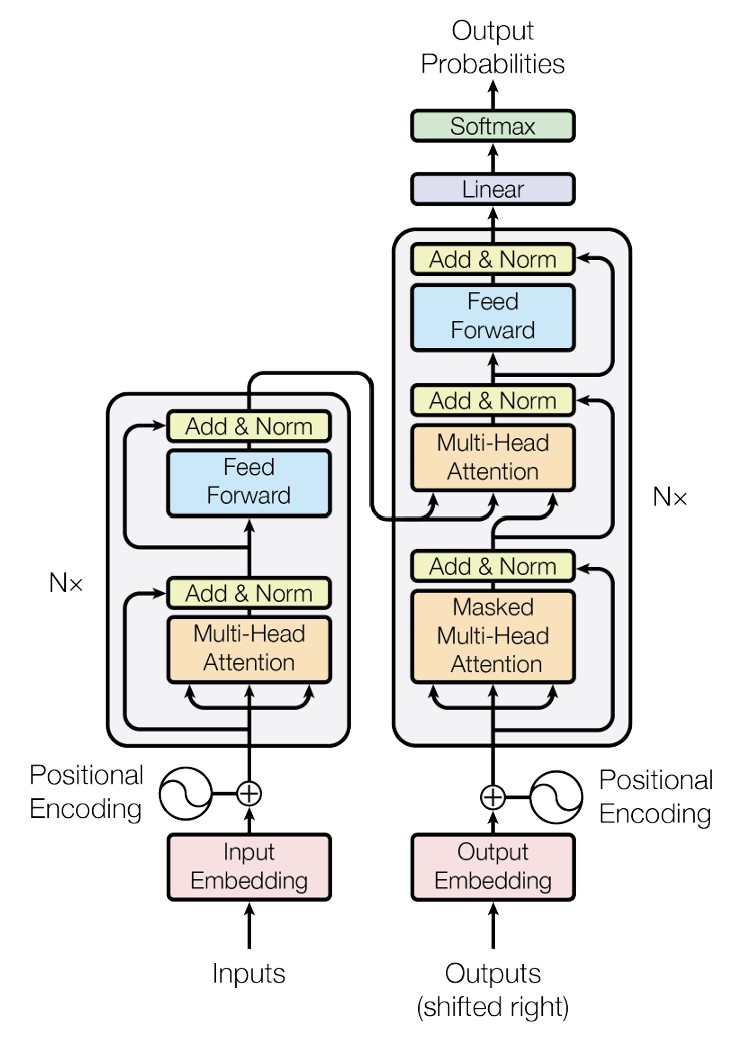
\includegraphics[width=0.3\linewidth]{./figures/TransformerArchitecture.jpg}
    \caption{Transformer整体架构}
    \label{fig:TransformerArchitecture}
\end{figure}

\begin{figure}[H]
    \centering
    \begin{subfigure}[b]{0.45\textwidth}
        \centering
        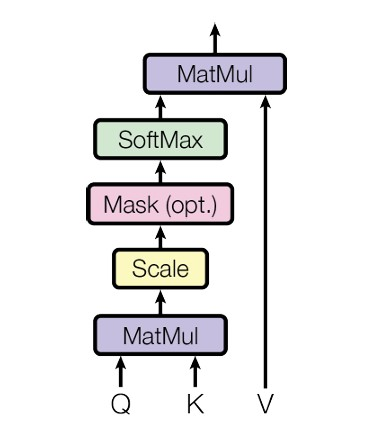
\includegraphics[width=0.5\linewidth]{./figures/ScaledDotProductAttention.jpg}
        \caption{注意力机制}
        \label{fig:ScaledDotProductAttention}
    \end{subfigure}
    \hfill
    \begin{subfigure}[b]{0.45\textwidth}
        \centering
        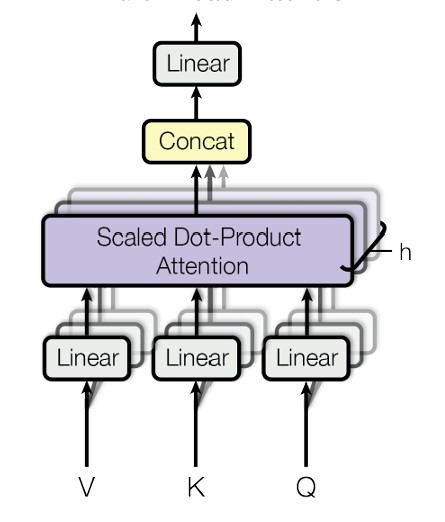
\includegraphics[width=0.5\linewidth]{./figures/MultiHeadAttetion.jpg}
        \caption{多头注意力机制}
        \label{fig:MultiHeadAttetion}
    \end{subfigure}
    \caption{Transformer机制图}
    \label{fig:transformermechanism}
\end{figure}

注意力机制通过计算输入序列中不同元素之间的相关性来为每个元素分配不同的权重。
其核心计算过程是缩放点积注意力(Scaled Dot-Product Attention),
如图\ref{fig:ScaledDotProductAttention}所示。
对于查询向量$\mathbf{Q}$,键向量$\mathbf{K}$,和值向量$\mathbf{V}$,其计算公式为:

\begin{equation}
    \text{Attention}(\mathbf{Q}, \mathbf{K}, \mathbf{V}) = \text{softmax}\left(\frac{\mathbf{QK}^T}{\sqrt{d_k}}\right)\mathbf{V}
\end{equation}
其中,$d_k$是键向量的维度,用于缩放点积以避免数值过大。

多头注意力机制是对注意力机制的扩展,它通过将输入序列映射到多个不同的子空间来捕获更多的特征,如图\ref{fig:MultiHeadAttetion}所示。
具体来说,输入$\mathbf{Q}$, $\mathbf{K}$, $\mathbf{V}$分别经过线性变换生成多个头,
每个头都执行独立的缩放点积注意力,然后将各头的输出拼接并通过线性变换得到最终输出:

\begin{equation}
    \text{MultiHead}(\mathbf{Q}, \mathbf{K}, \mathbf{V}) = \text{Concat}(\text{head}_1, \ldots, \text{head}_h)\mathbf{W}^O
\end{equation}
其中每个头的计算为:

\begin{equation}
    \text{head}_i = \text{Attention}(\mathbf{Q}\mathbf{W}_i^Q, \mathbf{K}\mathbf{W}_i^K, \mathbf{V}\mathbf{W}_i^V)
\end{equation}

由于Transformer不包含循环结构,为了引入序列信息,
位置编码(Positional Encoding)被添加到输入序列中。
位置编码是预先定义的,常用的是正弦和余弦函数生成的编码:

\begin{equation}
    \begin{aligned}
        \text{PE}_{(pos, 2i)} = \sin\left(\frac{pos}{10000^{2i/d_{model}}}\right)\\
        \text{PE}_{(pos, 2i+1)} = \cos\left(\frac{pos}{10000^{2i/d_{model}}}\right)
    \end{aligned}
\end{equation}
其中$pos$是位置,$i$是维度索引,$d_{model}$是模型的维度。

本次实验中的所构建的模型编码器和解码器的层数均为6层,原始输入与RNN相同,
训练过程的损失曲线如图\ref{fig:TransformerLossHistory}所示,
模型各层权重矩阵可视化结果以及文本生成结果见附录。
其中不使用调度器时损失值收敛于0.0049,使用调度器时损失值收敛于0.0091。
\begin{figure}[H]
    \centering
    \begin{subfigure}[b]{0.45\textwidth}
        \centering
        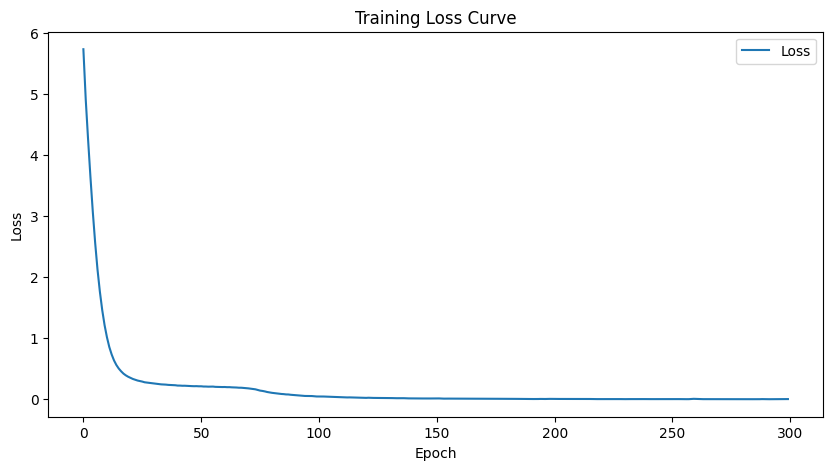
\includegraphics[width=\linewidth]{../output/transformer/no scheduler/loss history.png}
        \caption{不使用调度器}
        \label{fig:TransformerLossHistorynoscheduler}
    \end{subfigure}
    \hfill
    \begin{subfigure}[b]{0.45\textwidth}
        \centering
        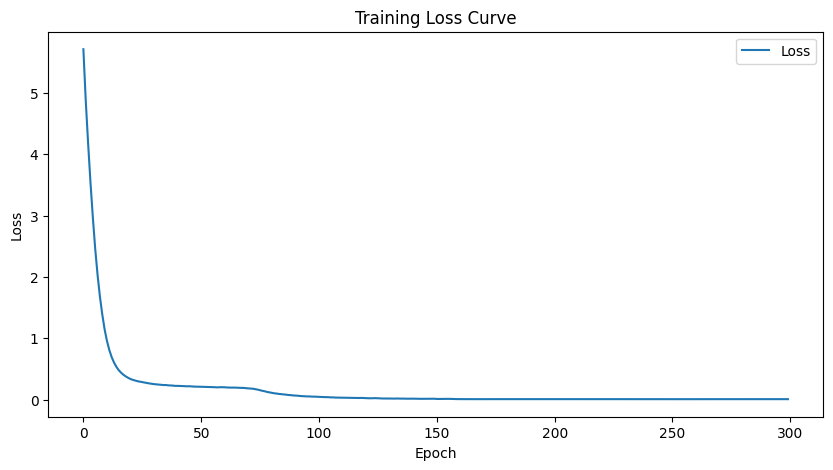
\includegraphics[width=\linewidth]{../output/transformer/with scheduler/loss history.png}
        \caption{使用调度器}
        \label{fig:TransformerLossHistorywithscheduler}
    \end{subfigure}
    \caption{损失曲线}
    \label{fig:TransformerLossHistory}
\end{figure}